\documentclass[a4paper,11pt]{article}
\pdfoutput=1 % if your are submitting a pdflatex (i.e. if you have
             % images in pdf, png or jpg format)

\usepackage{jcappub} % for details on the use of the package, please
                     % see the JCAP-author-manual

\usepackage[T1]{fontenc} % if needed
% \usepackage{subfig}
\usepackage[utf8]{inputenc}

\title{\boldmath The Core-Cusp Problem Revisited: ULDM vs. CDM}


%% %simple case: 2 authors, same institution
%% \author{A. Uthor}
%% \author{and A. Nother Author}
%% \affiliation{Institution,\\Address, Country}

% more complex case: 4 authors, 3 institutions, 2 footnotes
\author[1]{Emily Kendall}

% The "\note" macro will give a warning: "Ignoring empty anchor..."
% you can safely ignore it.

\affiliation[1]{Department of Physics, University of Auckland, Private Bag 92019, Auckland, New Zealand}

% e-mail addresses: one for each author, in the same order as the authors
\emailAdd{eken000@aucklanduni.ac.nz}




\abstract{The core-cusp problem of CDM has often been cited as motivation for the exploration of alternative dark matter models. Ultra-light dark matter is one such alternative, in which kiloparsec-scale Bose-Einstein condensates serve to flatten the density profiles of the central regions of dark matter halos. Recently, however, it has been suggested that ULDM may in fact exacerbate the core-cusp problem relative to CDM in some mass regimes. We further explore this idea, and find that current observational and simulation data are insufficient to draw concrete conclusions as to whether the CDM (excluding baryonic feedback) or ULDM models are better suited to describe the density profiles of dwarf galaxies.}



\begin{document}
\maketitle
\flushbottom

\section{TO DO}
\begin{itemize}
    \item remove x values from figure 1 
    \item acknowledgements
\end{itemize}


\section{Introduction}\label{sec:intro}

While it is widely agreed that non-baryonic dark matter constitutes the majority of the mass of the observable universe, its precise nature remains one of the most important open questions in theoretical physics today. Many models have been proposed to account for this non-baryonic matter, and among the most successful and widely promulgated is the WIMP model. While the WIMP model of dark matter has enjoyed extraordinary successes in the prediction of the large scale structure of the universe \cite{Springel:2005nw}, it has also suffered setbacks in the form of the so-called `small-scale crisis' \cite{Weinberg:2013aya}. One such small-scale problem arises due to tension between the predicted central density profiles of dark matter halos from CDM-only simulations and those inferred from observational data. While simulations tend to produce `cuspy' NFW-type central density profiles, which go like $1/r$ at small radii, observational data appears to favour flattened central cores \cite{REF} . This so called `core-cusp' problem has been the focus of much research in recent years \cite{Dutton:2018nop, Read:2018pft, Genina:2018}. 

The seriousness of the `core-cusp' problem is often disputed on the basis that the inclusion of baryonic physics within CDM simulations may alleviate the discrepancy in some cases \cite{Benitez-Llambay:2018}. Notwithstanding this ongoing contention, the `core-cusp' problem remains a motivating factor for the exploration of alternative models of dark matter in which tension with observational data is ameliorated through non-baryonic mechanisms. One such alternative model of dark matter which has been gaining traction is ultra-light dark matter (ULDM), also known variously as scalar-field dark matter, $\Psi$ dark matter, axion dark matter, BEC dark matter and fuzzy dark matter. A recent review is given in \cite{Hui:2016ltb}. In this model, the extremely light dark matter particle mass ($\mathcal{O}(\sim 10^{-22}eV)$) gives rise to a kiloparsec-scale de Broglie wavelength. Consequently, ultra-light dark matter exhibits novel wave-like behaviour on astrophysically relevant scales. Of particular interest is the ability of ULDM to form halos in which the inner core is described by a kilo-parsec scale Bose-Einstein condensate. The outer halo, meanwhile, is described by a virialised system of scalar particles with properties similar to standard CDM \cite{Schwabe:2016rze}. ULDM simulations have shown that the profiles of halo cores in this model match the family of solitonic ground state solutions to the Schrodinger-Poisson system, which have flat central densities \cite{Veltmaat:2018dfz}. Hence, without the inclusion of complicated baryonic physics, ULDM appears to be a natural candidate to resolve the core-cusp problem of CDM.

Despite this apparent success, it has recently been argued that in some mass regimes, the density profiles predicted by ULDM actually exacerbate the core-cusp problem in comparison to the NFW profiles characteristic of WIMP CDM \cite{Robles:2018fur}. Indeed, as the inner regions of ULDM halos are described by solitonic density profiles, they are subject to the mass scaling laws of the ground-state soliton solutions. Crucially, this means that as the mass contained within the central core increases, its radius decreases. For this reason, it is natural to expect that in the most massive cores, a large amount of mass is contained within a small radius. Hence, it is plausible that at small radii the internal mass of a heavy ULDM halo might exceed that of an `equivalent' NFW halo. The authors of \cite{Robles:2018fur} concluded that in comparison to observational data, the NFW profiles of CDM outperform ULDM profiles for dwarf galaxies with masses ($> M_h \sim 10^{11} M_{\odot}$). The purpose of this paper is to analyse the robustness of this conclusion when variation in the core-halo mass scaling relation of ULDM halos is taken into account. We find that under these circumstances, it cannot be concluded with any certainty that ULDM is outperformed by CDM at scales of $M_h \sim 10^{11}-10^{12} M_{\odot}$.

\section{ULDM profiles from simulations}

A number of numerical investigations have been undertaken into halo formation in the ULDM model, such as \cite{Schwabe:2016rze, Mocz:2017wlg, Lin:2018whl}. The numerical results suggest that the generic profile of a ULDM halo can be described by a solitonic core surrounded by a turbulent outer halo whose density profile falls off like $1/r^3$. We have independently obtained this generic profile from simulations utilising the publicly available PyUltraLight tool \cite{Edwards:2018ccc}. The results of one such simulation are shown in Figure \ref{fig:pul}. 

The profile shown in Figure \ref{fig:pul} was obtained through the merger of eight randomly positioned solitons whose masses were selected from a Gaussian distribution centred at 5000 code units. The simulation was run at $512^3$ for a duration of 0.05 code units, while the volume of the simulation region, also in code units, was $0.2^3$. For a ULDM particle mass of $10^{-22}\operatorname{eV}$, these figures correspond to individual progenitor mass $\sim 1.1*10^{10}\operatorname{M}_{\odot}$, duration $\sim 3.8 \operatorname{Gyr}$, and side length $\sim 7.7 \operatorname{kpc}$. The shape of the density profile of the resulting merger product is found to be qualitatively similar for larger/smaller masses, though the size of the solitonic core is subject to the inverse mass-radius scaling relation of the ground-state solution to the Schr{\"o}dinger-Poisson equations. So that the merger product is able to relax and eject mass from the inner region of the halo, PyUltraLight was modified to include a sponge at the simulation boundary, meaning that mass is not globally conserved. The duration of the simulation was chosen to be sufficiently long such that the mass-loss rate asymptotically approaches zero well before the end of the simulation. In this way the resulting halo represents a relaxed merger product. 

The left panel of Figure \ref{fig:pul} demonstrates the spherically-averaged density profile of the relaxed merger product over time. The inner region is solitonic, transitioning to a $1/r^3$ type profile between 3 and 4 times the core radius. While there is some time-dependence of the overall profile, it is largely stable. However, the right side panel demonstrates significant local fluctuations in the outer halo along any individual arbitrary direction. These local fluctuations should be taken into account when trying to fit halo profiles inferred from velocity data for astrophysical objects, as any given point may be deviate strongly from the global average profile. 



\begin{figure}
\begin{tabular}{cc}
{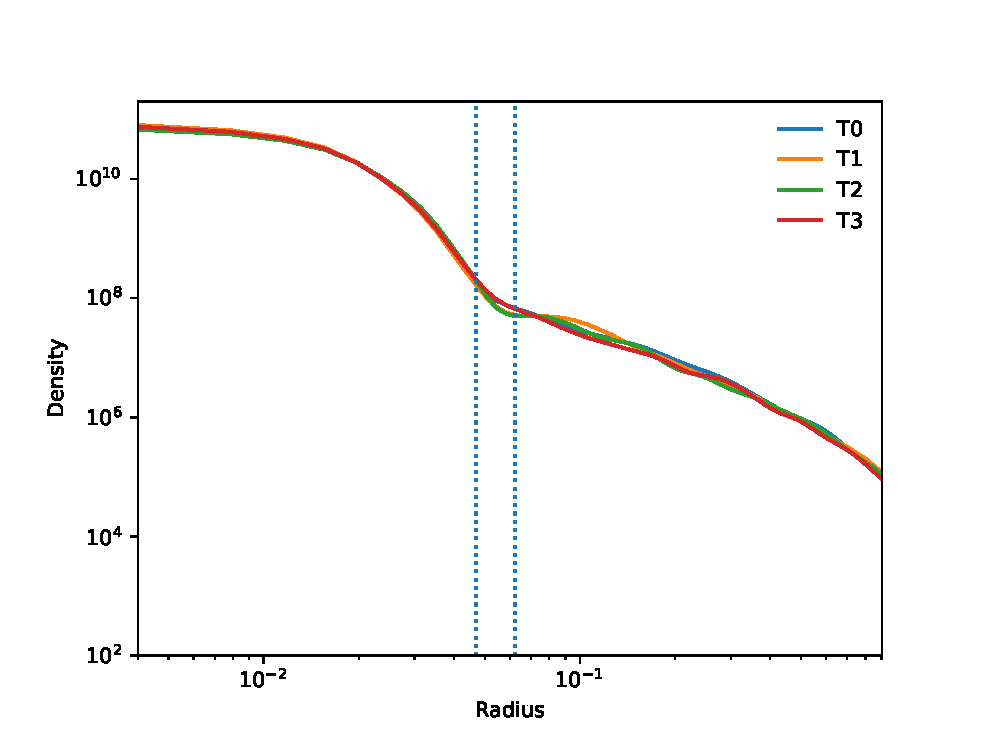
\includegraphics[scale = 0.55, trim={1.5cm 0 0 1cm}]{pics/combined3.eps}} &
{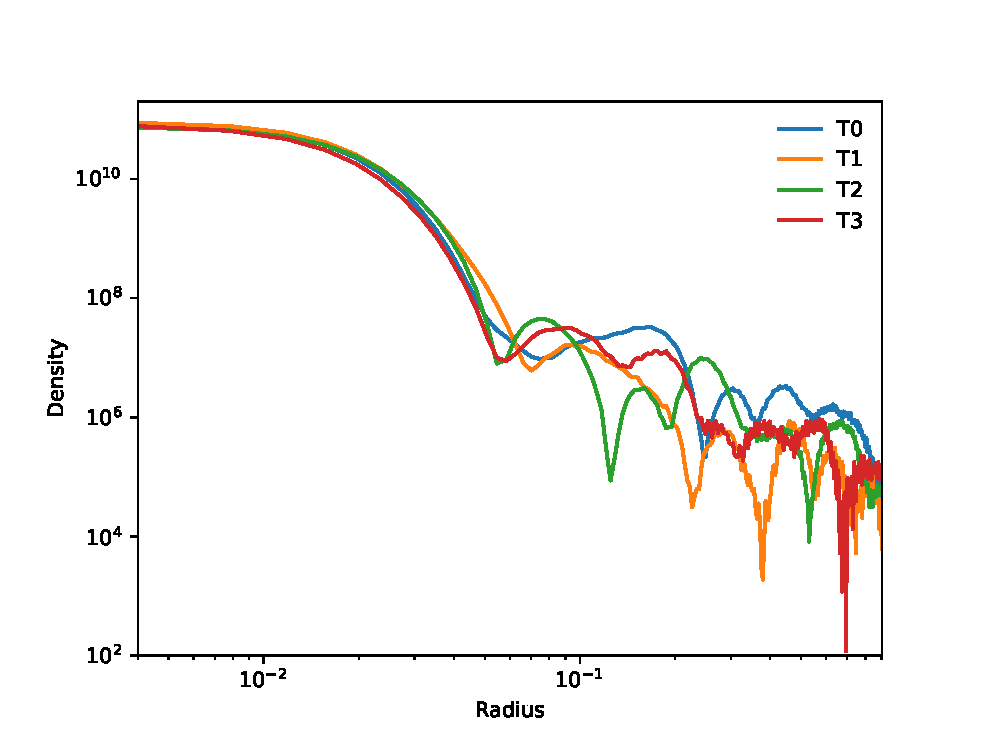
\includegraphics[scale = 0.55, trim={2cm 0 0 1cm}]{pics/singles.eps}}
\end{tabular}
\caption{Left: Spherically averaged density profile of merger product of 8 $\sim 5000$ code unit solitons. Vertical dotted lines represent 3 and 4 times the core radius (radius at half-maximum density). T1 to T4 represent snapshots at $0.85\times$total duration to $1.0 \times$ total duration. 
Right: Density profile along single arbitrary direction.}\label{fig:pul}
\end{figure}





\section{Semi-analytic models of dark matter halos and the ULDM core-halo mass relation}

\subsection{The NFW profile of CDM}

In order to contrast the performance of ULDM and CDM in terms of predicting astrophysical halo density profiles, it is important to establish a means by which halos from either model can be considered to be equivalent. To this end, it is useful to establish semi-analytic models to represent the archetypal profiles of each model. The NFW profile of CDM is widely recognised as a useful tool for modelling the generic properties of CDM halos \cite{Navarro:1995iw, Maccio:2008pcd}. This profile is given by
\begin{equation}\label{eq:nfw}
    \rho_{NFW}(r)=\frac{\rho_0}{\frac{r}{R_s}\left(1+\frac{r}{R_s}\right)^2}.
\end{equation}
Where the parameters $\rho_0$ and $R_s$ vary from halo to halo. It is clear from this equation that the mass of an NFW halo diverges if integrated to arbitrarily large radius. It is therefore necessary to prescribe a cutoff radius for integration in order to give a finite value for the mass. Typically, the virial radius is approximately determined using the spherical top-hat collapse model \cite{White:2000jv, Suto:2015jdt, Herrera:2017epn}. This simple model describes the collapse of a uniform spherical overdensity in a smooth expanding background. The collapse of the overdensity is halted when virial equilibrium is reached, and it is found that the resulting virial radius is that where the average internal density is given by $\Delta_c \rho_c(t)$. Here, $\Delta_c$ is a numerical factor of order $10^2$, while $\rho_c(t)$ is the critical density of the universe at time $t$. While different conventions exist for the choice of $\Delta_c$, we will choose the relatively common standard $\Delta_c = 200$ \cite{Richings:2018}. 

With the virial radius imposed as the cutoff for the physical extent of the halo, equation \ref{eq:nfw} completely specifies the density profile for given choices of $\rho_0$ and $R_s$. Thus, for any given virial mass, a range of corresponding NFW density profiles can be determined, where the choices of $\rho_0$ and $R_s$ are restricted by the mass-concentration-redshift relation evident in the results of N-body simulations \cite{Ludlow:2013vxa}. 

\subsection{The piecewise ULDM halo profile}

In order to compare generic CDM halos with their ULDM counterparts, it is necessary to prescribe a method by which, for a given virial mass, a range of suitable ULDM halos can be specified. The authors of \cite{Bullock} constructed a piecewise generic ULDM profile as
\begin{equation}\label{eq:piecewise}
     \rho(r)=
    \begin{cases}
      \rho_{sol}(r), & 0\leq r \leq r_{\alpha} \\
      \rho_{NFW}(r), & r_{\alpha}\leq r \leq r_{vir},
    \end{cases}
\end{equation}
where $\rho_{sol}(r)$ is the appropriately scaled density profile of the ground state soliton solution to the Schr{\"o}dinger-Poisson system of coupled differential equations, to be discussed shortly, and the densities of the solitonic and NFW pieces are matched at the transition radius $r_{\alpha}$.

To calculate the solitonic density profile, we must numerically solve for the spherically symmetric ground state solution to the dimensionless Schr{\"o}dinger-Poisson equations:
\begin{align}
    i\dot{\psi} &= -\frac{1}{2}\nabla^2\psi+\Phi\psi \\
    \nabla^2\Phi &= 4\pi \vert \psi\vert^2
\end{align}
Choosing the initial condition $\vert\psi(x=0)\vert = 1$, we can obtain the radial profile of $\psi$ using a fourth-order Runge-Kutta method \cite{Edwards:2018ccc}. From this we can construct the whole family of solutions for $\vert\psi(x=0)\vert = \gamma$ by making use of the scaling properties of the Schr{\"o}dinger-Poisson system. That is, if $\psi(x)$ represents our $\gamma = 1$ solution, then
\begin{equation}
    \psi'(x) = \gamma\psi(\sqrt{\gamma}x)
\end{equation}
is also a solution. Hence, we can simply scale the initial profile accordingly for arbitrary $\gamma$. Under this scaling, the dimensionless mass of the soliton is proportional to $\sqrt{\gamma}$, while the dimensionless radius is proportional to $1/\sqrt{\gamma}$. The dimensionless density $\vert\psi\vert^2$ and dimensionless radius $x$ can be transformed into dimensionful quantities by
\begin{align}
    \rho &= \mathcal{M}\mathcal{L}^{-3}\vert\psi\vert^2, \label{eq:density_conv} \\
    r &= \mathcal{L}x, \label{eq:mass_conv}
\end{align}
where
\begin{equation}\label{eq:length}
    \mathcal{L}=\left(\frac{8\pi\hbar^2}{3 m^2H_0^2\Omega_{m_0}}\right)^{\frac{1}{4}}\approx121\left(\frac{10^{-23}\operatorname{eV}}{m}\right)^{\frac{1}{2}}\operatorname{kpc},\label{eq:length}
\end{equation}

\begin{equation}\label{eq:mass}
    \mathcal{M}=\frac{1}{G}\left(\frac{8\pi}{3 H_0^2\Omega_{m_0}}\right)^{-\frac{1}{4}}\left(\frac{\hbar}{m}\right)^{\frac{3}{2}}\approx 7\times 10^7\left(\frac{10^{-23}\operatorname{eV}}{m}\right)^{\frac{3}{2}}\operatorname{M}_{\odot}.
\end{equation}
\\

To construct the ULDM halo profile in accordance with \ref{eq:piecewise}, we must determine the predicted central density, $\rho_c$ of a ULDM halo for a given virial mass, $M_{vir}$. In \cite{Robles:2018fur}, this is done by making use of the core-halo mass relation found by the authors of \cite{Schive:2014hza} from numerical simulations. In particular, we have that 
\begin{equation}
    \rho_c = 2.94*10^6 \operatorname{M}_{\odot}\operatorname{kpc}^{-3}\left(\frac{M_{vir}}{10^9 M_{\odot}}\right)^{4/3}m_{22}^{2}
\end{equation}
and 
\begin{equation}
    r_c = 1.6 \operatorname{kpc}\left(\frac{M_{vir}}{10^9 M_{\odot}}\right)^{-1/3}m_{22}^{-1},
\end{equation}
where $r_c$ is the radius at which the density drops to half its central value, and $m_{22}$ is defined as $m_{22} \equiv m / 10^{-22} \operatorname{eV}$. Here $m$ is the ULDM particle mass. 

While this precise scaling relation gives us a baseline prediction for the central density of a ULDM halo of a given virial mass, it is natural to expect, in analogy with the scatter in the concentration parameter of NFW profiles \cite{Maccio:2008pcd}, that there will in fact be a range of acceptable central densities for a given halo  mass. Indeed, inspection of the results of \cite{Schive:2014hza} indicates a scatter of up to $\pm 50\%$ from the theoretically predicted value of the core mass, $M_c$ (mass within $r_c$). Because of the small sample size of the data in \cite{Schive:2014hza}, as well as the fact that the halo masses considered cover only a limited range ($ M_{vir} \approx 10^8-10^{11} \operatorname{M}_{\odot}$), it is not possible to give precise values for the $1\sigma$  or $2 \sigma$ statistical deviations from the theoretical prediction of  $\operatorname{M}_c$. For the purposes of this analysis, therefore,  we will assume a scatter of $\pm 50\%$, with the caveat that data from future simulations will likely improve these statistics.

As acknowledged in \cite{Robles:2018fur}, not only is statistical variation in central soliton density expected, but also statistical variation in the radius at which the solitonic profile of the ULDM halo transitions into an NFW profile. This variation is captured by the parameter $\alpha$, such that the transition radius, $r_{\alpha}$, is given by $r_{\alpha} = \alpha r_c$, where $3 \leq \alpha \leq 4$.

With the allowances for statistical variation in both the central soliton density and the transition radius taken into account, we can now create a range of acceptable ULDM halo profiles for a given halo virial mass. To do this, we use the virial mass to predict $\rho_c$. Combined with an assumption for $\alpha$, the solitonic piece of the ULDM profile is then completely specified, and its mass can be calculated. From here, we can calculate the remaining mass which must be accommodated by the NFW tail of the ULDM profile, and by matching the densities of the NFW tail and the inner soliton at the transition radius, the values of the $R_s$ and $rho_0$ parameters of the ULDM profile NFW tail are fully constrained. 

\section{Comparison of ULDM and CDM halos for $\operatorname{M}_{vir} = 10^{11} -  10^{12} \operatorname{M}_{\odot}$}

Using the formalism above, we can compare the range of plausible ULDM halo profiles to that of NFW profiles for halos of masses $10^{11}$ and $10^{12} \operatorname{M}_{\odot}$. The results of these comparisons are shown in Figure \ref{fig:profiles}. The green lines represent the ULDM density profiles at the extreme ends of the $\operatorname{M}_c = \operatorname{M}_{cp} \pm 50 \% \operatorname{M}_{cp}$ range, where $\operatorname{M}_{cp}$ is the theoretical predicition for the core mass. Note that due to the scaling relations of the soliton solution to the Schr{\"o}dinger-Poisson relations, this mass range corresponds to a range of $ \gamma_p /4 \geq \gamma \leq 9\gamma_p/4$, where $\gamma_p$ is the theoretical prediction of the square root of the dimensionless central density. This large variation in the central density results in widely varying predictions for the overall ULDM profiles. Meanwhile the 1-$\sigma$ and 2-$\sigma$ ranges for NFW profiles with different concentrations are plotted with red and blue dots, respectively \cite{Maccio:2008pcd}. 

In keeping with \cite{Robles:2018fur}, we plot to a minimum radius of $r/r_vir = 10^{-4}$. We note in passing that for any $\operatorname{M}_{vir}$, the NFW halo density at small radii will inevitably exceed that of the ULDM halo, though the threshold for this transition may be arbitrarily small, and not observationally accessible. Furthermore, as in \cite{Robles:2018fur} we contrast the  results corresponding to differing assumptions for the ULDM particle mass, namely $m_{22} = 0.8 - 2.5$.



\begin{figure}
\begin{tabular}{cc}
{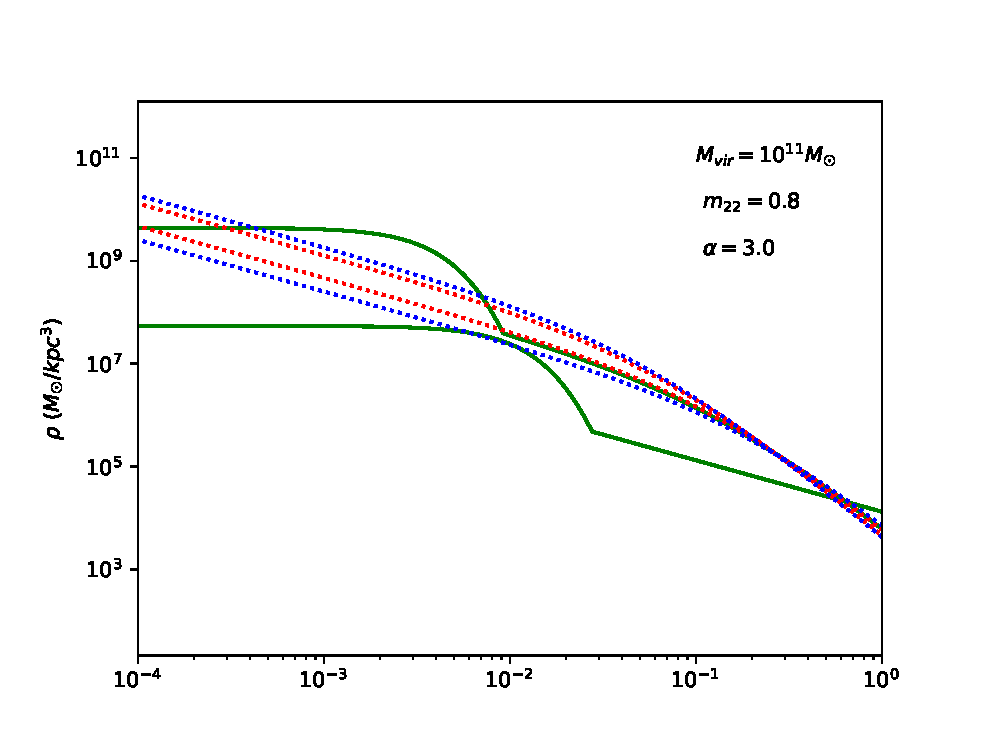
\includegraphics[width = 3.1in, trim={2.1cm 0.5cm 0cm 0.5cm}]{pics/11_8_3.eps}} &
{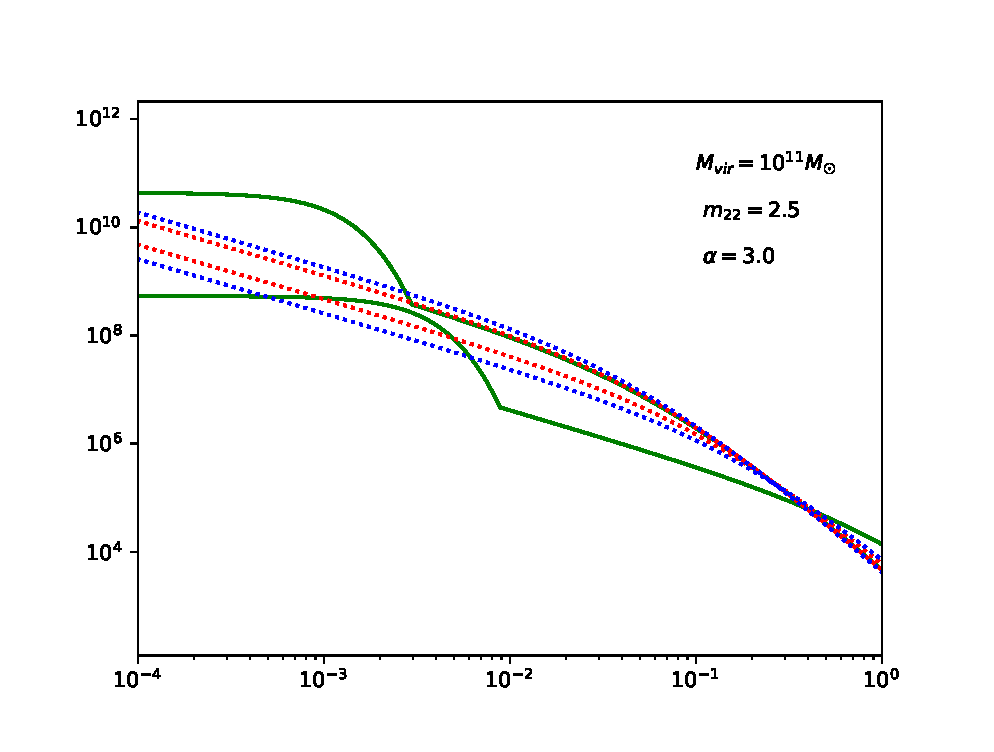
\includegraphics[width = 3.1in, trim={2.1cm 0.5cm 0cm 0.5cm}]{pics/11_25_3.eps}}\\
{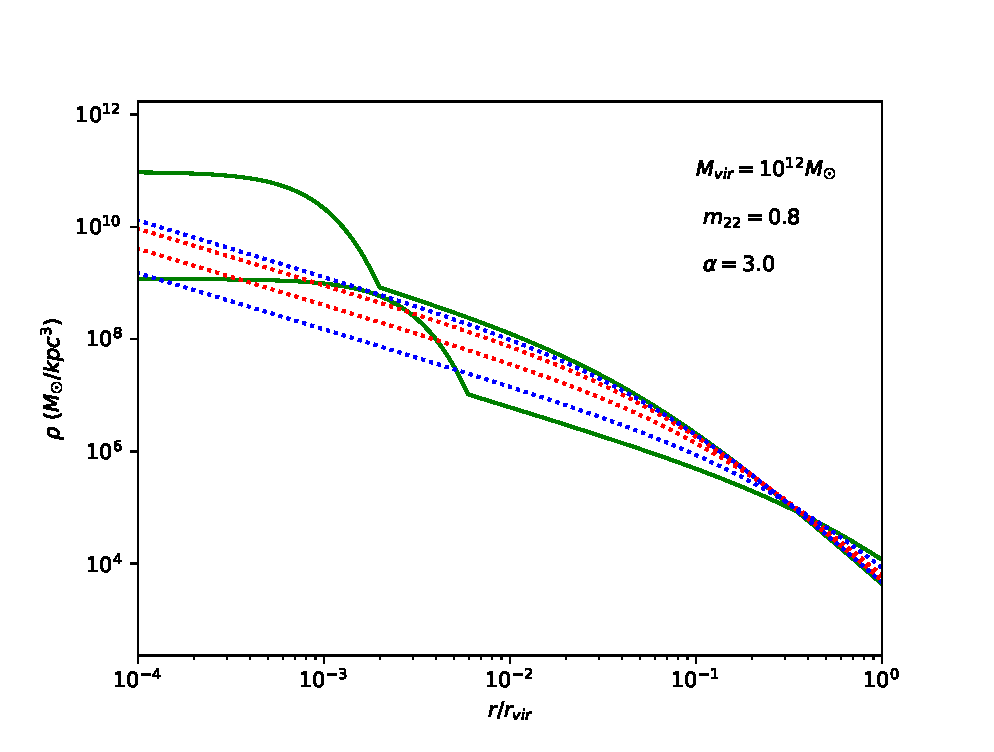
\includegraphics[width = 3.1in, trim={2.1cm 0.5cm 0cm 0.5cm}]{pics/12_8_3.eps}} &
{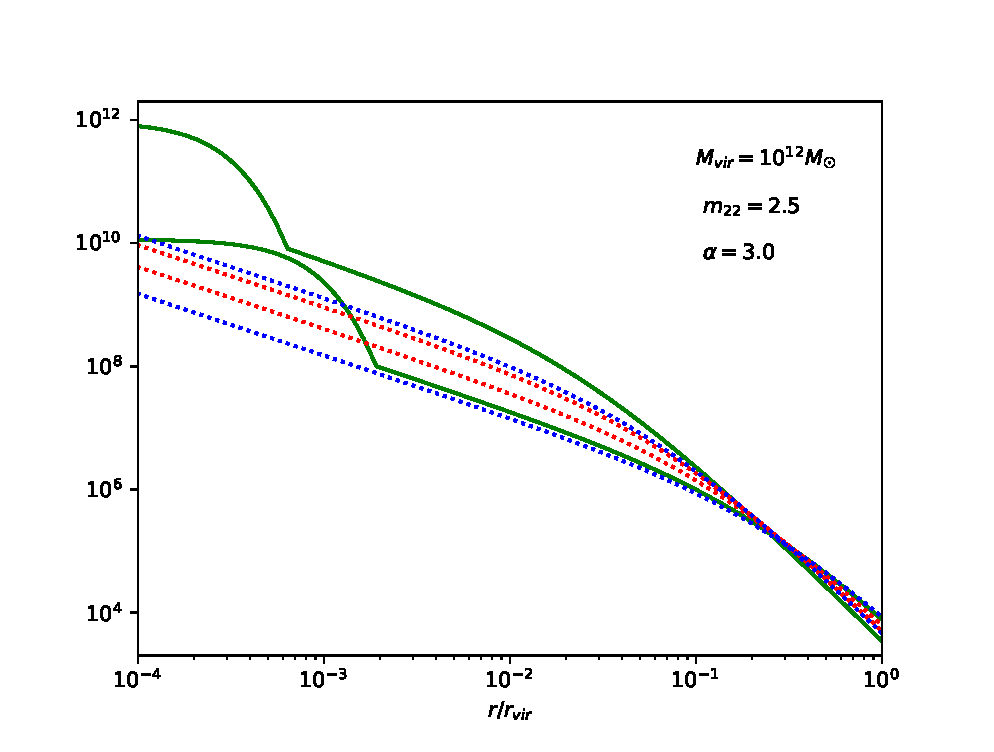
\includegraphics[width = 3.1in, trim={2.1cm 0.5cm 0cm 0.5cm}]{pics/12_25_3.eps}}
\end{tabular}
\caption{Density profiles as a function of radius (normalised to the virial radius) for ULDM and NFW halos of masses $10^{11}\operatorname{M}_{\odot}$ (top) and $10^{12}\operatorname{M}_{\odot}$ (bottom). The left panel represents the results for $m_{22} = 0.8$, while the right panel corresponds to $m_{22}=2.5$. In all cases the transition radius has been taken to be $r_{\alpha} = 3*r_c$, as its value does not affect the value of the ULDM central density.}\label{fig:profiles}
\end{figure}


We turn our attention now to the core-cusp discrepancy. From Figure \ref{fig:profiles} we see that for halos of mass $10^{11}\operatorname{M}_{\odot}$ there exists a significant band within the region bounded by the extremal ULDM profiles for which ULDM outperforms NFW.  Of course, plotting to smaller radii would amplify this apparent advantage. For halos of mass $10^{12}\operatorname{M}_{\odot}$, we see that for lower ULDM particle mass ($m_{22}=0.8$), the ULDM profiles are still able to outperform the NFW profiles, though at higher particle mass ($m_{22}=2.5$) the  NFW profiles tend to outperform the ULDM profiles in the range $10^{-4}\leq r/r_{vir} \leq 1$.

Of course, it is not the dark matter halo density profiles themselves which are directly obtained through astrophysical observations, rather it is the radial velocity distributions of tracer stars. In the following section, we will compare the theoretical velocity profiles to observational data from the SPARC database \cite{Lelli:2016zqa}, in order to see whether UDLM or NFW profiles lead to better consistency with data. 

\section{Comparison of velocity distributions to SPARC data}

In this section we will convert the density profiles of Figure \ref{fig:profiles} to their corresponding radial velocity distributions. We will then plot these distributions against observational data from the SPARC database. The velocity is given by
\begin{equation}
    V(r)^2 = \frac{4\pi G}{r}\int_0^r \rho(r')r'^2 dr',
\end{equation}
where (\cite{Sofue:2008wt})
\begin{equation}
    V^2 = V_{disk}^2 + V_{bulge}^2 + V_{gas}^2 + V_{halo}^2.
\end{equation}
The disk and bulge velocities in the SPARC database are given for $\Upsilon = 1 \operatorname{M}_{\odot}/\operatorname{L}_{\odot}$ at $3.6\operatorname{\mu m}$. However, the greatest source of uncertainty in mass modelling is the assumption for the stellar mass-to-light ratio, $\Upsilon_\star$ \cite{Lelli:2016zqa}. As in \cite{Robles:2018fur}, we will assume a constant value of $\Upsilon_\star = 0.2 \operatorname{M}_{\odot}/\operatorname{L}_{\odot}$ at $3.6\operatorname{\mu m}$, but acknowledge that this constitutes a non-trivial source of uncertainty in the results. It should also be noted that the there is significant uncertainty in the SPARC data itself, though the error bars are not plotted in the following graphs for ease of viewing. 

The SPARC database contains data photometric data for 175 galaxies, with maximum velocities spanning a range of over $200 \operatorname{kms}^{-1}$. For comparison to the theoretical velocity profiles of the $10^{11}\operatorname{M}_{\odot}$ halos, we have chosen only those candidates with maximum velocity $< 1.2\times 10^2 \operatorname{kms}^{-1}$. The comparisons are shown in Figures \ref{fig:velocity_11} and \ref{fig:velocity_12}.


\begin{figure}
\begin{tabular}{cc}
{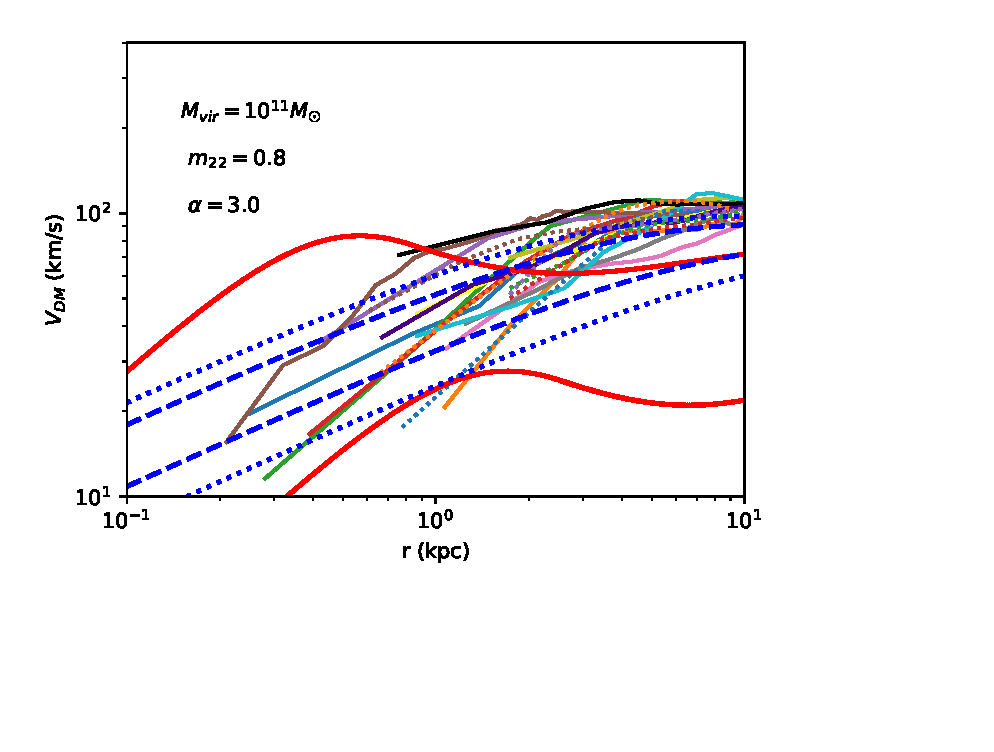
\includegraphics[scale = 0.65, trim={2.5cm 2.5cm 2.1cm 0.5cm}]{pics/v_11_8_3_paper.eps}} &
{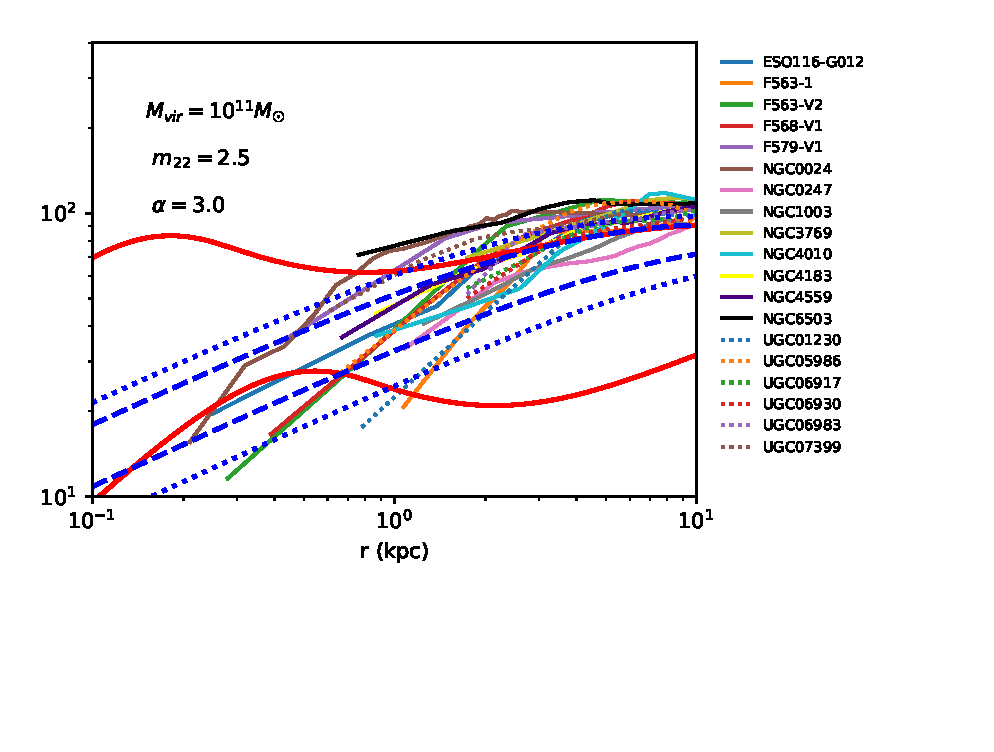
\includegraphics[scale = 0.65, trim={2.1cm 2.5cm 0cm 0.5cm}]{pics/v_11_25_3_paper.eps}}
\end{tabular}
\caption{Theoretical NFW and ULDM velocity profiles for $10^{11}\operatorname{M}_{\odot}$ halos plotted against SPARC data filtered by $V_{max} < 1.2 \operatorname{kms}^{-1}$. Red solid lines represent the extremal ULDM velocity profiles, while  blue dashed and dotted lines represent the 1-$\sigma$ and 2-$\sigma$ NFW bands, respectively. Results are shown for ULDM particle mass $m_{22} = 0.8$ (left) and $m_{22} = 2.5 $ (right).}\label{fig:velocity_11}
\end{figure}

From Figure 2, we see that neither the NFW profile nor the ULDM profile for $10^{11}\operatorname{M}_{\odot}$ appear to show good agreement with the data. While the core-cusp problem is not necessarily exacerbated in the ULDM case, ULDM profiles which roughly fit the data at low radii fall short at larger radii. This problem is exacerbated at larger values of $\alpha$. It should be noted, however, that at small radii where the proportion of baryonic matter is expected to be highest, inaccuracies in the assumptions of the stellar mass to light ratio will have a non-negligible effect. For this reason it is difficult to determine with certainty which model, if either, is a better fit to the data.

While the SPARC database does not contain any cases for which the velocity is significantly below $10^2\operatorname{kms}^{-1}$ at $10 \operatorname{kpc}$, it would appear that the ULDM profiles for the $10^{11}\operatorname{M}_{\odot}$ halos may provide a better fit to data in a lower velocity regime at this radius. 


In Figure \ref{fig:velocity_12}, we show the comparison of the theoretical profiles for the $10^{11}\operatorname{M}_{\odot}$ halos with SPARC data satisfying $1.55 \operatorname{kms}^{-1}\leq V_{max}\leq 2.0 \operatorname{kms}^{-1}$.


\begin{figure}
\begin{tabular}{cc}
{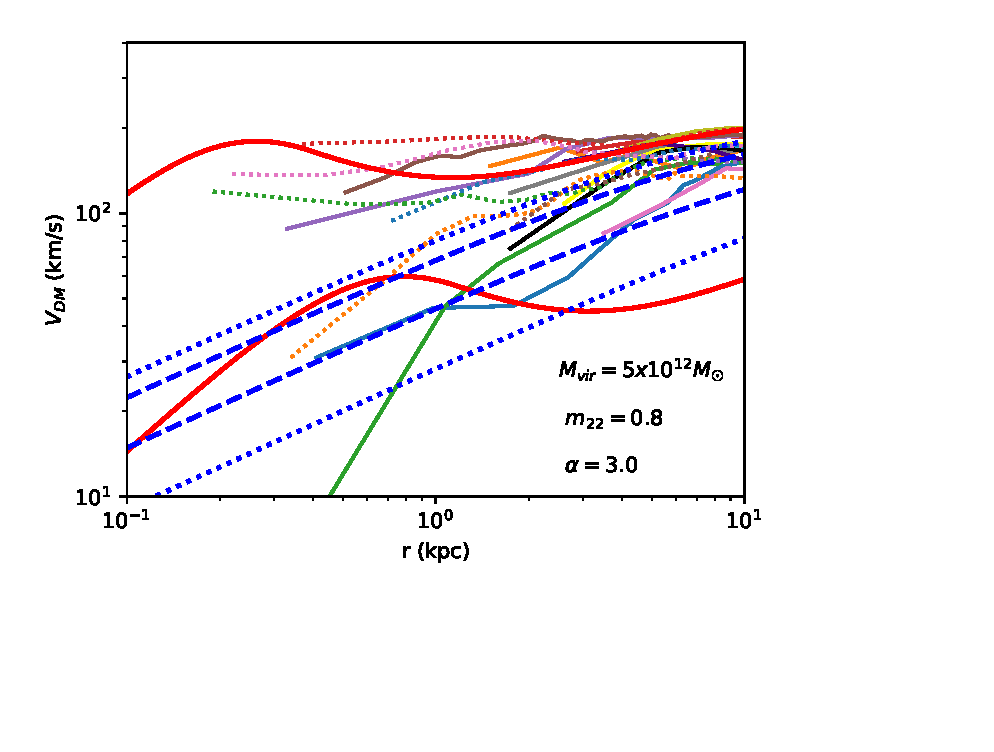
\includegraphics[scale = 0.65, trim={2.5cm 2.5cm 2.1cm 0.5cm}]{pics/velocity.eps}} &
{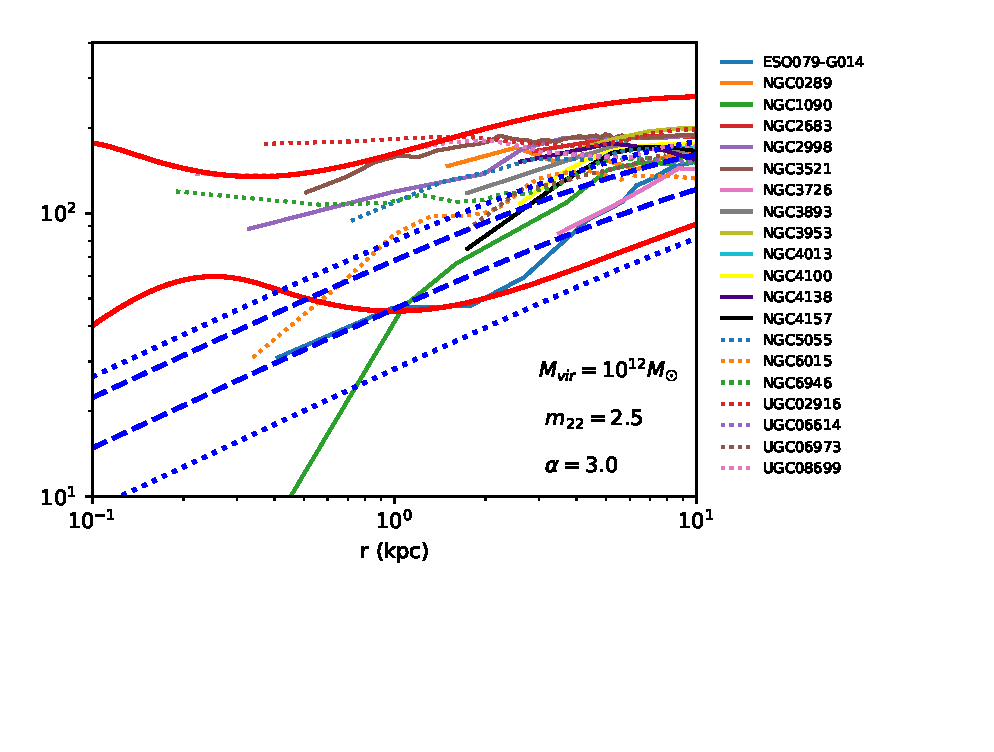
\includegraphics[scale = 0.65, trim={2.1cm 2.5cm 0cm 0.5cm}]{pics/v_12_25_3_paper.eps}}
\end{tabular}
\caption{Theoretical NFW and ULDM velocity profiles for $10^{12}\operatorname{M}_{\odot}$ halos plotted against SPARC data filtered by $1.55 \operatorname{kms}^{-1}\leq V_{max}\leq 2.0 \operatorname{kms}^{-1}$. Red solid lines represent the extremal ULDM velocity profiles, while  blue dashed and dotted lines represent the 1-$\sigma$ and 2-$\sigma$ NFW bands, respectively. Results are shown for ULDM particle mass $m_{22} = 0.8$ (left) and $m_{22} = 2.5 $ (right).}\label{fig:velocity_12}
\end{figure}



As for the $10^{11}\operatorname{M}_{\odot}$ case, neither the ULDM nor the NFW profiles appear to provide a particularly convincing fit to the data. In saying this, it must be recognised that there is significant variation in the trends in the data itself, so it would be difficult to find a universally applicable profile. Interestingly, however, there are a number of galaxies in this sample set which have flatter velocity profiles within the plotted range, such as NGC6946, UGC02916, and UGC08699. For these cases, the ULDM profile appears to provide a better fit, however more observational data would be required to confirm this. 

While the ULDM profiles predicted for $10^{11}$ and $10^{12} \operatorname{M}_{\odot}$ halos at $m_{22} = 0.8 - 2.5$ do not provide convincing fits to  the SPARC data, it is interesting to consider models with a slightly lower ULDM particle mass. In particular, if we consider $m_{22} = 0.1$, corresponding to $m = 10^{-23} \operatorname{eV}$, we find a much improved fit to the data. This is shown in Figure \ref{fig:velocity_23}. It should be noted, however, that a ULDM particle mass of this magnitude is in tension with constraints from the Lyman-$\alpha$ forest \cite{Amendola:2005ad}, as well as high-redshift UV luminosity function comparisons \cite{Bozek:2014uqa}. 

\\
\begin{figure}
\centering
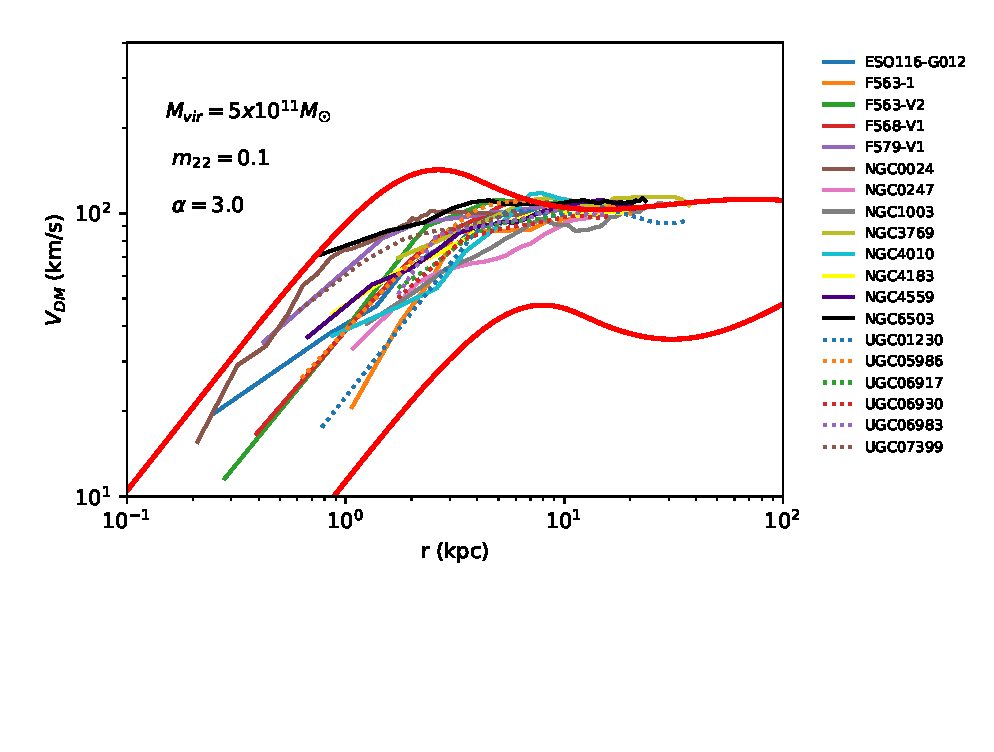
\includegraphics[scale = 0.7, trim={0cm 2.5cm 1cm 0.35cm}]{pics/best_match.eps} 
\caption{Range of theoretical ULDM profiles for a halo of mass $5\times 10^{11}\operatorname{M}_{\odot}$ and virial radius 200kpc with $m_{22} = 0.1$. Also plotted are the SPARC data satisfying $V_{max}\leq 1.2 \operatorname{kms}^{-1}$.}\label{fig:velocity_23}
\end{figure}


\section{Conclusions}

While the ULDM model has gained popularity as a means by which to resolve the contentious core-cusp problem of CDM, there exist cases in which theoretical ULDM profiles have higher densities than their NFW counterparts at observationally relevant radii in the interior of massive dwarf galaxies. However, given the apparent spread in the predicted ULDM core-halo mass relation \cite{Schive:2014hza}, there exists a significant range of plausible central densities for a halo of any given mass. In some circumstances this can mitigate the apparent core-cusp discrepancy. 

Comparison of theoretical ULDM and NFW profiles to photometric data from the SPARC database yields inconclusive results, as neither ULDM nor NFW profiles provide a particularly good fit to the data in the ranges $10^{11}\operatorname{M}_{\odot}\leq \operatorname{M}_{vir} \leq 10^{12}\operatorname{M}_{\odot}$ and $0.8 \leq m_{22} \leq 2.5$. Interestingly, however, a better fit to the lower velocity SPARC data is obtained from a ULDM profile where $m_{22} = 0.1$ and $\operatorname{M}_{vir} = 5\times 10^{11}\operatorname{M}_{\odot}$. While this ULDM particle mass appears to be in tension with current constraints \cite{Amendola:2005ad, Bozek:2014uqa}, a number of differing constraints on the ULDM particle mass have been proposed, with a lack of universal consensus \cite{Armengaud:2017nkf}.

It is clear that more data, both from simulations and astrophysical observations, is required to fully explore the applicability of the ULDM model of dark matter. A larger volume of photometric data with improved uncertainties and covering a greater halo mass range would be of tremendous benefit. Indeed, it is reasonable to expect a vast amount of new data becoming available in the near future, as a number of extensive surveys are undertaken \cite{Simon:2019kmm}. In addition, cosmological structure formation simulations for ULDM models continue to be an active area of research \cite{Lin:2018whl, Clough:2018exo, Mocz:2015sda}, and we can expect an improvement on the statistics surrounding the core-halo mass-redshift relation in future. Thus, while this preliminary work is somewhat inconclusive, it motivates further analyses of this kind in future as available datasets advance. 




\acknowledgments

This is the most common positions for acknowledgments. A macro is
available to maintain the same layout and spelling of the heading.





\bibliographystyle{JHEP-mod}
\bibliography{refs} 


\end{document}
